\graphicspath{{./figures/capitolo3/}}
\lstset{inputpath = ./programs/capitolo3}
\pgfplotstableset{search path = ./tables/capitolo3}

\chapter{Metodi lineari multistep}
Nel capitolo precedente abbiamo simulato sistemi dinamici
a tempo discreto tramite delle semplici sostituzioni in avanti.
Per poter trattare numericamente sistemi dinamici a tempo continuo,
di cui ci occuperemo più avanti a partire dal capitolo 5,
è necessario invece scegliere un'adeguata tecnica di discretizzazione,
ossia un procedimento che associa a un sistema dinamico continuo un analogo
sistema discreto in modo tale da preservarne sia gli aspetti quantitativi
delle dinamiche, sia gli aspetti qualitativi.
%La qualità del processo di discretizzazione verrà valutata sia da un punto
%di vista quantitativo (tramite l'errore di troncamento locale),
%sia da un punto di vista qualitativo (tramite varie nozioni di stabilità).
In questo capitolo andremo ad analizzare una delle famiglie più
importanti di metodi numerici per la soluzione di equazioni differenziali
ordinarie: quella dei cosiddetti \emph{metodi lineari multistep}.
Consideriamo il problema di Cauchy
\begin{equation}\label{eq:problema-di-cauchy}
\left\{
\begin{aligned}
y'(t)  &= f(t,y(t)) \quad \text{per ogni $t \in [t_0,T]$}, \\
y(t_0) &= y_0 \in \R^m.
\end{aligned}
\right.
\end{equation}
Qualunque problema ai valori iniziali per equazioni differenziali
ordinarie può essere scritto in questa forma, anche se potrebbe
rendersi necessaria l'introduzione di variabili ausiliarie.
Affinché abbia senso parlare di metodi numerici per la sua soluzione,
è necessario innanzitutto accertarsi che il
problema~\eqref{eq:problema-di-cauchy} sia ben posto.
A tal fine, un'ipotesi sufficiente è quella di chiedere che la funzione
$f$ sia continua e globalmente lipschitziana rispetto al secondo argomento:

\begin{defi}
Una funzione $f(t,y) \colon \R \times \R^m \to \R^m$ si dice
\emph{globalmente lipschitziana} rispetto alla variabile $y$
(in modo uniforme rispetto a $t$) se esiste una costante $L > 0$ tale che
\[
\norm{f(t,y_1)-f(t,y_2)} \leq L \norm{y_1-y_2}
\quad \text{per ogni $t \in \R$ e per ogni $y_1,y_2 \in \R^m$.}
\]
\end{defi}

\begin{teor}[Buona posizione globale]
Consideriamo il problema di Cauchy \eqref{eq:problema-di-cauchy}.
Se la funzione $f(t,y)$ è continua e globalmente lipschitziana rispetto
alla variabile $y$, allora esiste ed è unica la soluzione
$y(t) \colon [t_0,T] \to \R^m$.
Inoltre tale soluzione dipende in modo continuo
dai dati iniziali $y_0$ (rispetto alla norma $L^\infty$).
\end{teor}

\noindent Vista l'importanza di quest'ultimo risultato, supporremo per tutto
il capitolo che la funzione $f$ sia continua e globalmente lipschitziana
con costante di Lipschitz $L$.

Per arrivare a discretizzare il problema \eqref{eq:problema-di-cauchy},
è necessario in primo luogo discretizzare il dominio temporale $[t_0,T]$,
cioè sostituirlo con un insieme finito di nodi
\[
t_0 < t_1 < \ldots < t_{N-1} < t_N = T.
\]
È in corrispondenza di questi nodi che andremo ad approssimare
i valori della soluzione esatta continua~$y(t)$ con una successione finita $\{y_i\}$:
\[
y_0 \approx y(t_0),
\quad y_1 \approx y(t_1),
\quad \cdots,
\quad y_{N-1} \approx y(t_{N-1}),
\quad y_N \approx y(t_N) = y(T).
\]
Per semplicità, limitiamoci al caso di nodi equispaziati:
\[
t_i = t_0 + ih
\quad \text{per ogni $i = 0,\dots,N$,} \quad h = \frac{T-t_0}{N}.
\]
La costante $h$ è detta \emph{passo temporale}.
Il legame tra i diversi valori $y_i$ è dato dalla
discretizzazione dell'equazione differenziale $y'(t) = f(t,y(t))$.
È qui che entra in gioco la definizione di \emph{metodo lineare multistep}:
\begin{defi}
Sia $\alpha_k \neq 0$. Si dice \emph{metodo lineare a $k$ passi}
il problema ai valori iniziali discreto
\begin{equation}\label{eq:metodo-lmf}
\left\{
\begin{aligned}
& \sum_{i=0}^k \alpha_i y_{n+i} = h \sum_{i=0}^k \beta_i f(t_{n+i},y_{n+i})
\quad \text{per ogni $n=0,\dots,N-k$}, \\
& \, \text{$y_0,\dots,y_{k-1}$ fissati in $\R^m$}.
\end{aligned}
\right.
\end{equation}
\end{defi}
\noindent Senza perdita di generalità, si può sempre supporre $\alpha_k = 1$
(basta dividere per $\alpha_k$). Inoltre, affinché il metodo sia effettivamente
a $k$ passi (e non un numero inferiore), si richiede che $\alpha_0 \neq 0$,
oppure $\beta_0 \neq 0$. Il problema \eqref{eq:metodo-lmf} può essere scritto
in forma più compatta introducendo i polinomi
\[
\rho(z) \deq \sum_{i=0}^k \alpha_i z^i,
\quad \sigma(z) \deq \sum_{i=0}^k \beta_i z^i,
\]
detti \emph{polinomi caratteristici} del metodo lineare multistep.
Infatti, indicando con $E$ l'operatore di scorrimento in avanti
e con $f_i$ il valore di $f$ in $(t_i,y_i)$,
il problema \eqref{eq:metodo-lmf} equivale a
\begin{equation} \label{eq:metodo-lmf-rho-sigma}
\left\{
\begin{aligned}
& \rho(E) y_n = h \sigma(E) f_n \quad \text{per ogni $i=0,\dots,N-k$}, \\
& \, \text{$y_0,\dots,y_{k-1}$ fissati in $\R^m$}.
\end{aligned}
\right.
\end{equation}
In base al valore di $\beta_k$, i metodi lineari multistep sono
detti \emph{espliciti} oppure \emph{impliciti}.
Se $\beta_k = 0$, il valore $y_{n+k}$ può essere calcolato con facilità
a ogni iterazione tramite sostituzioni in avanti:
\[
y_{n+k} = - \sum_{i=0}^{k-1} \alpha_i y_{n+i}
        + h \sum_{i=0}^{k-1} \beta_i f(t_{n+i},y_{n+i})
        \eqd g_n.
\]
In questo caso il metodo è detto \emph{esplicito}.
Se invece $\beta_k \neq 0$, il valore $y_{n+k}$ dev'essere calcolato
a ogni iterazione tramite la soluzione dell'equazione generalmente non lineare
\begin{equation}\label{eq:equazione-nonlineare-lmf-implicito}
y - h \beta_k f(t_{n+k},y) = g_n
\end{equation}
nell'incognita vettoriale $y$. In questo caso il metodo è detto \emph{implicito}
e non è chiaro a priori se il problema \eqref{eq:metodo-lmf} ammetta
soluzione o se questa sia unica. Per fortuna, dato che la nonlinearità
può essere resa arbitrariamente piccola limitando il passo temporale $h$,
vale il seguente risultato:
\begin{teor}
Esiste un passo temporale $h$ uniforme rispetto a $n$ al di sotto del quale
l'equazione \eqref{eq:equazione-nonlineare-lmf-implicito} ha sempre soluzione,
e tale soluzione è unica.
\end{teor}
\begin{proof}
Basta assicurarsi che $h \abs{\beta_k} L$ sia minore di 1, così da poter
applicare il teorema di punto fisso di Banach alla funzione 
$G(y) = h \beta_k f(t_{n+k},y) + g_n$.
\end{proof}

\section{Proprietà quantitative}
Non tutte le scelte dei coefficienti $\alpha_i$ e $\beta_i$
danno luogo a metodi lineari multistep validi, cioè in grado
di approssimare la soluzione del problema \eqref{eq:problema-di-cauchy}.
Un requisito fondamentale è il seguente:
\begin{defi}
Un metodo lineare a $k$ passi si dice \emph{convergente} se
\[
\lim_{h \to 0} \; \max_{0 \leq n \leq N} \bigl\{ \norm{y(t_n)-y_n} \bigr\} = 0.
\]
Inoltre, se esiste $p > 0$ per cui
\[
\max_{0 \leq n \leq N} \bigl\{ \norm{y(t_n)-y_n} \bigr\} = O(h^p),
\]
l'estremo superiore dei valori che $p$ può assumere in tale uguaglianza
(in realtà, un'inclusione) è detto \emph{ordine di convergenza} del metodo.
\end{defi}

Dato che la convergenza è un concetto globale,
non è facile stabilire in modo diretto se un particolare
metodo lineare multistep sia convergente o meno.
Più avanti vedremo una caratterizzazione della convergenza
a partire da due altre proprietà: la \emph{0-stabilità} e la \emph{consistenza}.
Iniziamo da quest'ultima:
\begin{defi}
Si dice \emph{errore locale di troncamento} la quantità ottenuta
sostituendo la soluzione esatta $y(t_i)$ al posto di $y_i$ nell'equazione
alle differenze che definisce un metodo lineare a $k$ passi:
\begin{equation} \label{eq:errore-locale-di-troncamento}
\tau_{n+k}
\deq \sum_{i=0}^k \alpha_i y(t_{n+i})
 - h \sum_{i=0}^k \beta_i f(t_{n+i},y(t_{n+i}))
\quad \text{per ogni $n=0,\dots,N-k$}.
\end{equation}
Se esiste $p \geq 0$ tale che
\[
\max_{0 \leq n \leq N-k} \norm{\tau_{n+k}} = O(h^{p+1}),
\]
allora il massimo valore intero che $p$ può assumere in tale uguaglianza
(in realtà, un'inclusione) è detto \emph{ordine} del metodo.
Un metodo lineare a $k$ passi si dice \emph{consistente} se ha ordine
almeno 1.
\end{defi}
\begin{teor}
Supponiamo che un metodo lineare a $k$ passi abbia ordine $p$.
Se $h \abs{\beta_k} L < 1$ e se vale l'\emph{ipotesi localizzante}
$y_n = y(t_n), \dots, y_{n+k-1} = y(t_{n+k-1})$, allora
\[
y(t_{n+k}) - y_{n+k} = \tau_{n+k} + O(h^{p+2}).
\]
\end{teor}
\noindent A meno di infinitesimi di ordine superiore, possiamo
quindi interpretare l'errore di troncamento locale $\tau_{n+k}$
come l'errore che si commetterebbe al passo $n$-esimo di un metodo multistep
se si partisse da valori esatti per i $k$ passi precedenti.

Dato che l'ordine di un metodo lineare a $k$ passi è una proprietà locale,
è possibile caratterizzare tale proprietà mediante la formula di Taylor
sotto forma di vincoli sui coefficienti $\alpha_i$ e $\beta_i$:
\begin{teor} \label{teor:ordine-lmf}
Un metodo lineare a $k$ passi ha ordine $p$ per ogni problema
\eqref{eq:problema-di-cauchy} con soluzioni di regolarità $C^{p+1}$
se e solo se i coefficienti $\alpha_i$, $\beta_i$ del metodo soddisfano
le seguenti identità:
\begin{equation} \label{eq:ordine-lmf}
\sum_{i=0}^k \alpha_i = 0,
\qquad \sum_{i=0}^k (i^j \alpha_i - j i^{j-1} \beta_i) = 0
\quad \text{per ogni $j = 1,\dots,p$.}
\end{equation}
\end{teor}
%\noindent Un metodo lineare multistep è dunque consistente se e solo se
%\[
%\sum_{i=0}^k \alpha_i = 0,
%\quad \sum_{i=0}^k (i \alpha_i - \beta_i) = 0.
%\]
\noindent Qual è il massimo ordine di un metodo lineare a $k$ passi?
Se il metodo è implicito abbiamo $2k+1$ gradi di libertà
$(\alpha_0,\dots,\alpha_{k-1},\beta_0,\dots,\beta_k)$,
quindi possiamo senz'altro ottenere metodi di ordine $2k$ in virtù
del teorema precedente (perché richiede $2k+1$ vincoli lineari).
In realtà si può dimostrare (grazie alla teoria delle matrici di Vandermonde
confluenti) che tutti i vincoli del teorema precedente sono linearmente
indipendenti, quindi esiste ed è unico il metodo lineare a $k$ passi
implicito di ordine $2k$, ma a parità di passi non possono esistere metodi
di ordine superiore. Nel caso di metodi espliciti abbiamo un vincolo aggiuntivo,
cioè $\beta_k = 0$, quindi l'ordine massimo sarà $2k-1$.
I polinomi caratteristici di questi metodi di ordine massimo sono riportati
per $k \leq 4$ nelle Tabelle \ref{tab:lmf-max-order-implicit-coefficients}
e \ref{tab:lmf-max-order-explicit-coefficients}.
Tali polinomi sono stati calcolati mediante il
Programma~\ref{prog:max-order-implicit} nel caso implicito
e il Programma~\ref{prog:max-order-explicit} nel caso esplicito.
I due programmi funzionano più o meno nello stesso modo:
entrambi risolvono in aritmetica esatta il sistema lineare
che si ottiene andando a imporre i vincoli del Teorema~\ref{teor:ordine-lmf},
con l'unica differenza che il secondo programma impone anche
il vincolo $\beta_k = 0$.

Purtroppo, si può dimostrare che questi metodi lineari multistep
di ordine massimo non sono convergenti, a parte pochissime eccezioni
($k=1,2$ nel caso implicito, $k=1$ nel caso esplicito).
Nel caso generale abbiamo quindi a che fare con metodi lineari multistep
consistenti, ma non convergenti.
Il fatto è che non basta avere un errore locale di troncamento
\emph{asintoticamente piccolo}: bisogna anche assicurarsi che gli errori
locali non vengano amplificati in modo eccessivo a ogni passo
(per esempio, è impossibile andare in convergenza se questi errori
crescono come una successione geometrica a $N$ termini con passo maggiore di 1).

Queste considerazioni ci portano in modo naturale a considerare altre
proprietà di un metodo lineare multistep, stavolta di tipo globale,
qualitativo e legate a questioni di stabilità.

\lstinputlisting[float=p,label=prog:max-order-implicit,
caption={Calcolo dei coefficienti $\alpha_i$ e $\beta_i$ del metodo lineare
a $k$ passi implicito di ordine $2k$.}]{max_order_implicit_coefficients.m}

\begin{table}[p]
\caption{Polinomi caratteristici dei metodi lineari
a $k$ passi impliciti di ordine $2k$.}
\label{tab:lmf-max-order-implicit-coefficients}
\vspace*{-2.5ex}
\begin{equation*}
\begin{array}{cll}
\toprule
k & \rho(z) & \sigma(z) \\
\midrule
1 & z-1                       & (1/2)z+(1/2) \\
2 & z^2-1                     & (1/3)z^2+(4/3)z+(1/3) \\
3 & z^3+(27/11)z^2-(27/11)z-1 & (3/11)z^3+(27/11)z^2+(27/11)z+(3/11) \\
4 & z^4+(32/5)z^3-(32/5)z-1   & (6/25)z^4+(96/25)z^3+(216/25)z^2+(96/25)z+(6/25) \\
\bottomrule
\end{array}
\end{equation*}
\end{table}

\begin{table}[p]
\caption{Polinomi caratteristici dei metodi lineari
a $k$ passi espliciti di ordine $2k-1$.}
\label{tab:lmf-max-order-explicit-coefficients}
\begin{equation*}
\begin{array}{cll}
\toprule
k & \rho(z) & \sigma(z) \\
\midrule
1 & z-1                             & 1 \\
2 & z^2+4z-5                        & 4z+2 \\
3 & z^3+18z^2-9z-10                 & 9z^2+18z+3 \\
4 & z^4+(128/3)z^3+36z^2-64z-(47/3) & 16z^3+72z^2+48z+4 \\
\bottomrule
\end{array}
\end{equation*}
\end{table}

\clearpage

\lstinputlisting[float=tp,label=prog:max-order-explicit,
caption={Calcolo dei coefficienti $\alpha_i$ e $\beta_i$ del metodo lineare
a $k$ passi esplicito di ordine $2k-1$.}]{max_order_explicit_coefficients.m}

\section{Zero-stabilità}
Abbiamo visto che, per valori di $h$ sufficientemente piccoli,
il problema \eqref{eq:metodo-lmf} ha un'unica soluzione.
Tuttavia, non è detto che tale problema sia ben posto,
cioè che la soluzione $\{y_i\}$ sia stabile rispetto a una perturbazione
dei dati iniziali $y_0,\dots,y_{k-1}$.
Inoltre, nel paragrafo precedente abbiamo visto come un metodo
consistente non sia necessariamente convergente.
In entrambi i casi, l'ipotesi mancante è quella di \emph{zero-stabilità}:

\begin{defi}
Un metodo lineare multistep caratterizzato dai polinomi $(\rho,\sigma)$
si dice \emph{0-stabile} se $\rho$ è un polinomio di Von Neumann.
\end{defi}

\noindent La definizione appena data si può motivare considerando il problema
$y'(t) = 0$, $y(t_0)=y_0$.
Dato che $f(t,y) \equiv 0$, l'equazione alle differenze che si ottiene
discretizzando il problema con un metodo lineare multistep è
\[
\rho(E)y_n = 0.
\]
Questa è un'equazione lineare a coefficienti costanti, quindi
possiamo applicare il Teorema \ref{teor:sol-stabili-eq-alle-diff-lineare}:
la soluzione costante $y_n \equiv y_0$ è stabile se e solo se
$\rho(z)$ è un polinomio di Von Neumann.
Dunque, affinché il problema discreto \eqref{eq:metodo-lmf} sia ben posto,
bisogna come minimo chiedere che un metodo lineare multistep sia
0-stabile.

È un fatto notevole che la 0-stabilità sia in realtà sufficiente a garantire
la convergenza di un metodo lineare multistep, a patto che sia consistente:

\begin{teor}
Sia $\hat{f}_n = f(t_n,y(t_n))$.
Allora $e_n \deq y(t_n) - y_n$ soddisfa l'\emph{equazione dell'errore}
\begin{equation}\label{eq:equazione-dell-errore-lmf}
\rho(E) e_n - h \sigma(E) (\hat{f}_n-f_n) = \tau_{n+k}
\end{equation}
\end{teor}

\begin{proof}
Basta sottrarre l'equazione \eqref{eq:metodo-lmf-rho-sigma}
dalla \eqref{eq:errore-locale-di-troncamento}.
\end{proof}

\begin{teor}\label{teor:ordine-convergenza-lmf}
Un metodo lineare a $k$ passi consistente e 0-stabile è convergente.
Più precisamente, se il metodo ha ordine $p$,
e se $\norm{e_i} = O(h^r)$ per ogni $i = 0,\dots,k-1$, allora
\[
\norm{e_n} = O(h^{\min(p,r)}) \quad \text{per ogni $n = k,\dots,N$.}
\]
\end{teor}

%Il Teorema \ref{teor:ordine-convergenza-lmf}
\noindent Questo teorema suggerisce
(anche se, di fatto, non implica) che l'ordine di convergenza di
un metodo lineare multistep possa essere limitato dagli errori sui
dati iniziali $e_0, \dots, e_{k-1}$.
In effetti, si può dimostrare che tale limitazione è veramente presente,
e che pertanto è indispensabile calcolare in modo accurato i valori iniziali
mancanti $y_1, \dots, y_{k-1}$ affinché un metodo lineare multistep
raggiunga il suo massimo ordine di convergenza.

Più avanti passeremo in rassegna le varie possibilità per il calcolo
dei valori iniziali; prima, però, commentiamo l'aspetto computazionale
della 0-stabilità.
Un metodo efficace per verificare la 0-stabilità di un metodo lineare
multistep consiste nell'applicare il secondo criterio di Schur
(Teorema \ref{teor:schur2}) al polinomio caratteristico $\rho$.
Alla fine del paragrafo \ref{sec:schur}, avevamo visto le difficoltà legate
all'implementazione di tale criterio in aritmetica inesatta.
Inoltre, un metodo lineare multistep consistente soddisfa
necessariamente la condizione $\rho(1) = 0$ (prima identità
nella \eqref{eq:ordine-lmf}), quindi abbiamo la certezza
che in questo contesto la stabilità di $\rho$ sia sensibile anche alla
minima perturbazione. Abbiamo pertanto implementato il secondo criterio
di Schur nel Programma \ref{prog:is-von-neumann} avendo cura di utilizzare
esclusivamente l'aritmetica esatta per i calcoli. Per fortuna,
le operazioni aritmetiche in MATLAB supportano in modo trasparente operandi
razionali, quindi si sono rese necessarie solamente un numero minimo di
modifiche rispetto al Programma \ref{prog:is-schur}.

A conferma di quanto affermato nel paragrafo precedente, cioè
che i metodi lineari a $k$ passi di ordine massimo non possono essere
utilizzati in pratica, abbiamo riportato nelle
Tabelle \ref{tab:lmf-max-order-implicit-0-stability}
e \ref{tab:lmf-max-order-explicit-0-stability}
l'esito del secondo criterio di Schur applicato ai loro polinomi
caratteristici $\rho$ (calcolati in aritmetica esatta):
si vede chiaramente che, a parte poche eccezioni (solo tre),
questi metodi non sono 0-stabili, e quindi danno luogo a discretizzazioni mal poste.

Appurato che i metodi lineari a $k$ passi di ordine massimo non
sono in generale 0-stabili, viene spontaneo chiedersi quale sia il massimo
ordine che un metodo 0-stabile possa avere. Il seguente teorema
ci dice che è necessario rinunciare a circa metà dei gradi di libertà
sui coefficienti $\alpha_i$ e $\beta_i$:

\begin{teor}[Prima barriera di Dahlquist]
Sia $p$ l'ordine di un metodo lineare a $k$ passi 0-stabile.
Allora, se $k$ è dispari, $p \leq k+1$, altrimenti $p \leq k+2$.
\end{teor}

\lstinputlisting[float=p,label=prog:is-von-neumann, caption={Algoritmo
ricorsivo basato sul secondo criterio di Schur.}]{is_von_neumann.m}

\begin{table}[p]
\caption{Zero-stabilità dei metodi lineari
a $k$ passi impliciti di ordine $2k$.}
\label{tab:lmf-max-order-implicit-0-stability}
\vspace*{-2.5ex}
\begin{equation*}
\begin{array}{cll}
\toprule
k & \rho(z) & \text{\code{is\_von\_neumann}} \\
\midrule
1 & z-1                       & \text{\code{true}}  \\
2 & z^2-1                     & \text{\code{true}}  \\
3 & z^3+(27/11)z^2-(27/11)z-1 & \text{\code{false}} \\
4 & z^4+(32/5)z^3-(32/5)z-1   & \text{\code{false}} \\
5 & z^5+(1625/137)z^4+(2000/137)z^3-(2000/137)z^2-(1625/137)z-1 & \text{\code{false}} \\
\bottomrule
\end{array}
\end{equation*}
\end{table}

\begin{table}[p]
\caption{Zero-stabilità dei metodi lineari
a $k$ passi espliciti di ordine $2k-1$.}
\label{tab:lmf-max-order-explicit-0-stability}
\begin{equation*}
\begin{array}{cll}
\toprule
k & \rho(z) & \text{\code{is\_von\_neumann}} \\
\midrule
1 & z-1                             & \text{\code{true}}  \\
2 & z^2+4z-5                        & \text{\code{false}} \\
3 & z^3+18z^2-9z-10                 & \text{\code{false}} \\
4 & z^4+(128/3)z^3+36z^2-64z-(47/3) & \text{\code{false}} \\
5 & z^5+(475/6)z^4+(700/3)z^3-100z^2-(575/3)z-(131/6) & \text{\code{false}} \\
\bottomrule
\end{array}
\end{equation*}
\end{table}

\section{Assoluta stabilità}
Nel paragrafo precedente abbiamo visto che metodi consistenti e 0-stabili
forniscono una soluzione numerica $\{y_n\}_{n = 0,\dots,N}$ che tende
punto per punto alla soluzione esatta $y(t)$ nel limite $h \to 0$.
Tuttavia, ci sono buone ragioni per cui, nella pratica, bisogna accontentarsi
di un valore di $h$ fissato. Innanzitutto, un algoritmo può eseguire solo
un numero finito di operazioni, quindi il limite $h \to 0$ non può essere
raggiunto per motivi computazionali. In secondo luogo, l'intervallo di
integrazione potrebbe essere illimitato, o comunque crescere come $h^{-1}$.
Questo è tipico di problemi in cui si è interessati al raggiungimento
di una configurazione di equilibrio per tempi grandi. Un'ulteriore ragione
è che all'aumentare di $N$ numero di passi aumenta anche l'errore dovuto
all'aritmetica finita. Per tutte queste ragioni, è utile studiare l'equazione
dell'errore \eqref{eq:equazione-dell-errore-lmf} per valori di $h$ fissati.
Ovviamente il caso generale con $f$ non lineare è impossibile da trattare,
tuttavia è utile linearizzare il problema e studiare per lo meno il caso scalare
\begin{equation}\label{eq:equazione-di-test}
\left\{
\begin{aligned}
y'(t)  &= \lambda y(t) \quad \text{per ogni $t \geq t_0, \quad \Re(\lambda) < 0$}, \\
y(t_0) &= y_0 \in \R,
\end{aligned}
\right.
\end{equation}
in cui sappiamo che $y(t) = \exp(\lambda(t-t_0))y_0 \to 0$ per $t \to +\infty$,
visto il segno della parte reale di $\lambda$. L'equazione \eqref{eq:equazione-di-test}
è nota come \emph{equazione di test scalare}. Fissato un passo $h > 0$, sia
$y_n$ il risultato di $n$ iterazioni del metodo lineare caratterizzato dai
polinomi $(\rho,\sigma)$. Ci eravamo riproposti di studiare l'equazione
dell'errore \eqref{eq:equazione-dell-errore-lmf}, ma osserviamo che $y_n \to 0$
implica necessariamente $e_n \to 0$. Dunque possiamo limitarci allo studio
dell'equazione alle differenze che governa la dinamica discreta di $y_n$:
\[
\rho(E) y_n - h \sigma(E) (\lambda y_n) = 0.
\]
Il polinomio caratteristico di questa equazione è $\rho - q\sigma$,
con $q = h\lambda$.
Allora $y_n \to 0$ se e solo se $\rho - q \sigma$ è un polinomio di Schur,
e in tal caso si dirà che il metodo lineare multistep è \emph{assolutamente
stabile} in $q = h\lambda$.

\begin{defi}
Il polinomio $\rho - q\sigma$ è detto \emph{polinomio di stabilità} del metodo.
L'insieme
\[
\mathcal{D} = \{ q \in \C \mid \rho - q \sigma \text{ è un polinomio di Schur} \}
\]
è detto \emph{regione di assoluta stabilità} del metodo.
Un metodo lineare multistep si dice \emph{A-stabile} se
$\C^- \subseteq \mathcal{D}$, cioè se è in grado di riprodurre tutte le
dinamiche asintoticamente stabili dell'equazione di test al variare
di $\lambda$ in $\C^- = \{ z \in \C \mid \Re(z) < 0 \}$.
Un metodo lineare multistep si dice \emph{perfettamente A-stabile}
se $\mathcal{D} = \C^-$, cioè se la dinamica discreta è asintoticamente
stabile in tutti e soli i casi in cui anche la dinamica continua lo è.
\end{defi}

\noindent La proprietà di assoluta stabilità, per quanto desiderabile,
impone purtroppo limiti severi all'ordine di un metodo lineare multistep:

\begin{teor}[Seconda barriera di Dahlquist] \label{teor:seconda-barriera-dahlquist}
La regione di assoluta stabilità di un metodo lineare multistep
esplicito è un insieme limitato, quindi non esistono metodi espliciti
assolutamente stabili. Inoltre, l'ordine massimo di un metodo lineare
multistep assolutamente stabile è al più 2.
\end{teor}

\noindent Questo risultato negativo ci obbliga quindi a rinunciare
all'assoluta stabilità se desideriamo utilizzare un metodo lineare
multistep di ordine elevato. Ha senso pertanto chiedersi quanto sia
grande la regione di assoluta stabilità: a parità di ordine di
convergenza sono preferibili metodi con una regione più ampia%
\footnote{In realtà, anche la forma della regione di assoluta
stabilità è molto importante.}, perché permettono di utilizzare un passo $h$
maggiore e di raggiungere quindi prima la configurazione di equilibrio
associata a una dinamica assolutamente stabile.

A meno che il polinomio di stabilità non abbia grado particolarmente basso,
è difficile dare una descrizione esplicita della regione di assoluta stabilità
di un metodo lineare multistep. Da un punto di vista numerico,
si potrebbe pensare di utilizzare il primo criterio di Schur
per campionare a tappeto $\C$, stabilendo così in ogni punto $q$
se $q$ appartenga o meno a $\mathcal{D}$. Questo approccio di forza bruta,
oltre ad avere dei seri problemi di implementazione (come facciamo a
campionare $\C$ con un numero finito di punti?), non è in realtà necessario.
È possibile infatti trovare una parametrizzazione esplicita del
bordo $\partial \mathcal{D}$:

\begin{defi}[Boundary locus]
Si dice \emph{boundary locus} di un metodo lineare multistep caratterizzato
dai polinomi $(\rho,\sigma)$ la curva chiusa
\[
\Gamma = \left\{ \frac{\rho(e^{i\theta})}{\sigma(e^{i\theta})}
\Bigm| \theta \in [0,2\pi] \right\}.
\]
Nel caso in cui esista $\theta \in [0,2\pi]$ tale che $\sigma(e^{i\theta})$
si annulla, si può comunque pensare a $\Gamma$ come una curva chiusa
sulla sfera di Riemann $\hat{\C}$.
\end{defi}

\begin{teor}
Sia $\mathcal{D}$ la regione di assoluta stabilità di un metodo lineare
multistep, e sia $\Gamma$ il suo boundary locus. Allora vale l'inclusione
(potenzialmente stretta) $\partial \mathcal{D} \subseteq \Gamma$.
\end{teor}

\begin{proof}
Questa dimostrazione dipende in modo cruciale dal fatto che le radici
del polinomio di stabilità $\rho - q \sigma$ sono funzioni continue di $q$.
Sia $q \in \partial \mathcal{D}$. Allora il polinomio di stabilità
non può avere alcuna radice di modulo maggiore di 1, altrimenti
per continuità $q$ apparterrebbe all'aperto
$\C \setminus \overline{\mathcal{D}}$.
Analogamente, il polinomio di stabilità non può avere tutte le radici
di modulo minore di 1, altrimenti per continuità $q$ apparterrebbe
all'aperto $\mathcal{D}$. Pertanto, l'unica possibilità rimasta è che
$\rho - q \sigma$ abbia almeno una radice di modulo 1, diciamo $z$.
Allora esiste $\theta \in [0,2\pi)$ tale che $z = \exp(i\theta)$
e quindi
\[
\rho(e^{i\theta}) - q \sigma(e^{i\theta}) = 0
\quad \Longrightarrow \quad q \in \Gamma. \qedhere
\]
\end{proof}

\noindent Le idee utilizzate in questa dimostrazione permettono di ottenere
un risultato ancora più forte, cioè che la regione di assoluta stabilità è data
dall'unione (potenzialmente vuota) di alcune componenti connesse dell'insieme
$\C \setminus \Gamma$. Pertanto, un modo pratico ed efficiente per individuare
$\mathcal{D}$ consiste nel disegnare la curva chiusa $\Gamma$,
scegliere (anche a occhio) un punto $q_i$ in ogni componente connessa
$\mathcal{C}_i$ di $\C \setminus \Gamma$ e infine unire tutte le componenti
connesse $\mathcal{C}_i$ per cui $\rho - q_i \sigma$ sia un polinomio di Schur.
Di solito, $\mathcal{D}$ è un insieme connesso, ed è uguale all'unica
componente connessa di $\C \setminus \Gamma$ che contiene un intorno
sinistro dello zero (a meno che $\mathcal{D}$ non sia vuoto).

\section{Aspetti computazionali}

Scrivere un programma in grado di risolvere in modo approssimato il problema
di Cauchy \eqref{eq:problema-di-cauchy} per mezzo di un metodo lineare
multistep significa essenzialmente risolvere il problema discreto
\eqref{eq:metodo-lmf} in aritmetica finita.
Se $\beta_k = 0$, cioè se il metodo è esplicito,
l'equazione alle differenze
\[
y_{n+k} = - \sum_{i=0}^{k-1} \alpha_i y_{n+i}
        + h \sum_{i=0}^{k-1} \beta_i f(t_{n+i},y_{n+i})
        \eqd g_n.
\]
può essere risolta tramite sostituzioni in avanti, mentre se $\beta_k \neq 0$,
cioè se il metodo è implicito, abbiamo visto che per trovare $y_{n+k}$
a ogni passo bisogna risolvere il sistema non lineare
\begin{equation} \label{eq:equazione-nonlineare-lmf-implicito-2}
G_n(y) \deq y - h \beta_k f(t_{n+k},y) - g_n = 0
\end{equation}
nella variabile vettoriale $y$ (quindi un sistema con $m$ incognite scalari).
La dimostrazione di esistenza e unicità di una soluzione a tale equazione
non lineare, basata sul teorema di punto fisso di Banach,
suggerisce la possibilità di utilizzare un metodo di punto fisso
per risolvere il sistema \eqref{eq:equazione-nonlineare-lmf-implicito-2}.
Questo approccio, senz'altro possibile, non è però il più indicato, per due motivi.

In primo luogo, le iterazioni di punto fisso hanno convergenza globale, ma
tipicamente lenta, mentre in questo contesto sarebbe preferibile una convergenza
rapida (così da ridurre il costo computazionale), anche se locale, perché
a ogni passo del metodo lineare multistep abbiamo una buona approssimazione
di $y_{n+k}$ data da $y_{n+k-1}$, che possiamo usare come valore d'innesco
del metodo iterativo.
In secondo luogo, il metodo di punto fisso richiede la limitazione sul passo
$h \abs{\beta_k} L < 1$, che in alcuni casi può essere piuttosto severa
(per esempio, se il problema è \emph{stiff}) e di fatto vanifica molti
dei vantaggi nell'uso di metodi impliciti rispetto a metodi espliciti dello
stesso ordine (per esempio, le migliori proprietà di stabilità che consentono
di adottare passi grandi nel caso di problemi dissipativi).

Alla luce di queste considerazioni, si potrebbe allora pensare di risolvere
il sistema \eqref{eq:equazione-nonlineare-lmf-implicito-2} per mezzo del metodo
di Newton. Tuttavia, il calcolo della matrice jacobiana di $G_n(y)$
e la soluzione di un relativo sistema lineare a ogni iterazione del metodo
hanno un costo computazionale eccessivo, che nella pratica non giustifica
il beneficio della velocità di convergenza quadratica.

Un buon compromesso, allora, consiste nell'uso del \emph{metodo di Newton stazionario}
(o \emph{metodo delle corde}), cioè di una variante del metodo di Newton che
richiede il calcolo della matrice jacobiana $J$ solamente nel corso della
prima iterazione, e poi riutilizza la stessa matrice $J_0$ per tutte le
iterazioni successive. In questo modo, anche la soluzione dei sistemi lineari
diventa più veloce, perché è possibile calcolare la fattorizzazione $LU$
della matrice jacobiana una volta per tutte e da lì in poi utilizzare
soltanto solutori per matrici triangolari, con costo computazionale $O(m^2)$
anziché $O(m^3)$.
Si può dimostrare, purtroppo, che il metodo di Newton stazionario perde
la velocità di convergenza quadratica nel corso delle iterazioni, che
a un certo punto tornerà a essere lineare (perché $J_0$ non converge alla
jacobiana di $G_n(y)$ in $y_{n+k}$).
Tuttavia, ci sono due fattori che giocano a nostro favore.
Il primo è che non ha nessun senso risolvere il sistema
\eqref{eq:equazione-nonlineare-lmf-implicito-2} con un errore su $y$
significativamente minore dell'errore locale di troncamento del metodo
lineare multistep, perché l'errore $\abs{y(t_{n+k})-y_{n+k}}$ a ogni passo è
dato sostanzialmente dalla somma di questi due (più gli errori sui
$k$ valori $y_n, \dots, y_{n+k-1}$ precedenti e quelli dovuti all'aritmetica
finita, ovviamente). Pertanto, non è detto che la velocità di convergenza lineare
si manifesti prima di aver già raggiunto il criterio di arresto sulle
iterate (per quanto spiegato nel paragrafo dedicato all'analisi del metodo
delle secanti, è una buona idea utilizzare un criterio misto, cioè sia
assoluto che relativo). Alla luce del Teorema \ref{teor:ordine-convergenza-lmf},
la tolleranza del criterio di arresto è bene che sia scelta in modo da
essere minore di $h^{p+1}$, con $p$ ordine del metodo.

Il secondo motivo per cui il metodo di Newton stazionario funziona bene
in pratica è che il valore di innesco del metodo può essere scelto in modo
conveniente utilizzando un metodo esplicito economico (per esempio, il
metodo di Eulero), in modo da avere una matrice jacobiana $J_0$
il più vicino possibile alla jacobiana di $G_n(y)$ in $y_{n+k}$
e ritardare così l'avvento del regime lineare di convergenza (sempre che
il metodo esplicito non sia fonte di instabilità, però).

Alla luce di tutte queste considerazioni, abbiamo scritto il Programma
\ref{prog:lmf}, che realizza un generico metodo lineare multistep
dati i coefficienti $\alpha_i$ e $\beta_i$ in ingresso,
e i due programmi accessori \ref{prog:lmf-nonlinear-solver}
e \ref{prog:lmf-numerical-jacobian}, che si occupano rispettivamente
di risolvere il sistema \eqref{eq:equazione-nonlineare-lmf-implicito-2}
mediante il metodo di Newton stazionario e di calcolare la matrice jacobiana
spaziale di una funzione non lineare $f(t,y)$ mediante differenze finite
(in questo contesto, un errore relativo dell'ordine della radice
dell'epsilon di macchina è più che accettabile).
Commentiamo brevemente alcune scelte implementative.

In un metodo lineare a $k$ passi, il valore di $y_{n+k}$
è univocamente determinato dai $k$ valori precedenti $y_n,\dots,y_{n+k-1}$.
Pertanto, abbiamo potuto utilizzare una quantità di memoria costante
per memorizzare i valori $y_n, \, n = 0,\dots,N$ durante tutta l'esecuzione
dell'algoritmo: è stato sufficiente allocare $k$ vettori $y_0,\dots,y_{k-1}$
e poi ridurre modulo $k$ gli indici con cui si accede a tutti i vettori
$y_n$ successivi (linee di codice 34-38 nel Programma \ref{prog:lmf}).
Abbiamo adottato la stessa strategia anche per i vettori $f_n$,
che conviene tenere in memoria per evitare di ricalcolare $f(t_n,y_n)$
durante $k$ passi consecutivi.

Il Teorema \ref{teor:ordine-convergenza-lmf} e il commento seguente
ci dicono che il problema del calcolo dei $k-1$ valori iniziali
$y_1,\dots,y_{k-1}$ che non sono forniti dal problema di Cauchy
\eqref{eq:problema-di-cauchy} è una questione delicata.
Una possibilità, matematicamente elegante ma difficile da automatizzare
(a meno di appoggiarsi a pacchetti di calcolo simbolico) consiste nell'utilizzo
di uno sviluppo di Taylor di $y(t)$ con centro $t_0$.
Le derivate di $y(t)$ di ordine superiore al primo possono essere ottenute
differenziando $f(t,y(t))$, ma è chiaro che questo approccio è poco pratico
per metodi di ordine elevato: affinché l'errore su $y_1,\dots,y_{k-1}$
sia dell'ordine di $h^p$, infatti, sono richieste derivate fino all'ordine
$p-1$-esimo nella formula di Taylor.
Nel Programma \ref{prog:lmf}, linee 40-54, abbiamo preferito un approccio
numerico basato su metodi a un passo di tipo Runge-Kutta, metodi che
verranno esposti più avanti nel capitolo 8. Per esempio, un metodo Runge-Kutta
del 4° ordine (come \code{ode45}) ha errore di troncamento locale $O(h^5)$,
quindi è adatto a inizializzare metodi lineari multistep di ordine 5 o inferiore.

Per quanto riguarda l'analisi dell'assoluta stabilità di un metodo lineare
multistep, abbiamo scritto due programmi che permettono di individuare
la regione di assoluta stabilità $\mathcal{D}$ mediante la tecnica esposta
alla fine del paragrafo precedente: il Programma \ref{prog:lmf-plot-boundary-locus},
che disegna il boundary locus di un metodo dati i suoi coefficienti
$\alpha_i$ e $\beta_i$, e il Programma \ref{prog:lmf-is-in-stability-region},
che permette di stabilire se uno o più valori $q$ appartengono a $\mathcal{D}$
tramite il primo criterio di Schur applicato al polinomio di stabilità.

\clearpage

\lstinputlisting[label=prog:lmf, caption={Implementazione di un
generico metodo lineare multistep.}]{LMF.m}

\lstinputlisting[float=tbp, label=prog:lmf-nonlinear-solver, caption={Metodo di Newton
stazionario per metodi lineari multistep impliciti.}]{LMF_nonlinear_solver.m}

\lstinputlisting[float=tbp, label=prog:lmf-numerical-jacobian, caption={Calcolo numerico
di una matrice jacobiana mediante differenze finite.}]{numerical_jacobian.m}

\clearpage

\lstinputlisting[float=tbp, label=prog:lmf-plot-boundary-locus, caption={Visualizzazione
del boundary locus di un generico metodo lineare multistep.}]{plot_boundary_locus.m}

\lstinputlisting[float=tbp, label=prog:lmf-is-in-stability-region, caption={Test
di appartenenza alla regione di assoluta stabilit\`{a} di un metodo lineare
multistep.}]{is_in_stability_region.m}

\section{Metodi di Adams}

Passiamo ora alla definizione e all'analisi di alcuni tra i metodi lineari
multistep più importanti, compito che ci terrà occupati fino alla fine del capitolo.
I metodi lineari a $k$ passi con $\rho(z) = z^{k+1} (z-1)$ sono detti
\emph{metodi di Adams}. Osserviamo che questi metodi sono sempre 0-stabili,
perché $\rho$ è per costruzione un polinomio di Von Neumann.

I metodi di Adams espliciti sono detti \emph{metodi di Adams-Bashforth},
e si ottengono scegliendo i coefficienti $\beta_0,\dots,\beta_{k-1}$
in modo che il metodo raggiunga ordine $k$ (questo è possibile in virtù
del Teorema \ref{teor:ordine-lmf}). Per $k=1$ si ottiene il metodo
$y_{n+1} = y_n + h f(t_n,y_n)$, noto come \emph{metodo di Eulero esplicito}.
I polinomi caratteristici $\sigma$ dei metodi di ordine superiore sono riportati
nella Tabella \ref{tab:lmf-adams-bashforth-coefficients} fino a $k = 6$,
e sono stati calcolati per mezzo del Programma \ref{prog:adams-bashforth-coefficients}
(di cui abbiamo realizzato anche una versione in aritmetica esatta, che qui non riportiamo).

I metodi di Adams impliciti sono detti \emph{metodi di Adams-Moulton}, e si
ottengono scegliendo i coefficienti $\beta_0,\dots,\beta_k$ in modo che
il metodo raggiunga ordine $k+1$ (questo è possibile perché rispetto al
caso precedente abbiamo un grado di libertà aggiuntivo, associato a $\beta_k$).
Per $k=1$ si ottiene il metodo $y_{n+1} = y_n + (h/2) (f_{n+1}+f_n)$,
noto come \emph{metodo dei trapezi}.
I polinomi caratteristici $\sigma$ dei metodi di ordine superiore sono riportati
nella Tabella \ref{tab:lmf-adams-moulton-coefficients} fino a $k = 5$,
e sono stati calcolati per mezzo del Programma \ref{prog:adams-moulton-coefficients}.

\lstinputlisting[float=p, label=prog:adams-bashforth-coefficients,
caption={Calcolo dei coefficienti $\alpha_i$ e $\beta_i$ del metodo di
Adams-Bashforth a $k$ passi.}]{adams_bashforth_coefficients.m}

\begin{table}[p]
\caption{Polinomi caratteristici $\sigma$ di alcuni metodi di
Adams-Bashforth a $k$ passi.}
\label{tab:lmf-adams-bashforth-coefficients}
\vspace*{-2.5ex}
\begin{equation*}
\begin{array}{cl}
\toprule
k & \sigma(z) \\
\midrule
1 & 1 \\
2 & (3/2)z-(1/2) \\
3 & (23/12)z^2-(4/3)z+(5/12) \\
4 & (55/24)z^3-(59/24)z^2+(37/24)z-(3/8) \\
5 & (1901/720)z^4-(1387/360)z^3+(109/30)z^2-(637/360)z+(251/720) \\
6 & (4277/1440)z^5-(2641/480)z^4+(4991/720)z^3-(3649/720)z^2+(959/480)z-(95/288) \\
\bottomrule
\end{array}
\end{equation*}
\end{table}

\lstinputlisting[float=p, label=prog:adams-moulton-coefficients,
caption={Calcolo dei coefficienti $\alpha_i$ e $\beta_i$ del metodo di
Adams-Moulton a $k$ passi.}]{adams_moulton_coefficients.m}

\begin{table}[p]
\caption{Polinomi caratteristici $\sigma$ di alcuni metodi di
Adams-Moulton a $k$ passi.}
\label{tab:lmf-adams-moulton-coefficients}
\vspace*{-2.5ex}
\begin{equation*}
\begin{array}{cl}
\toprule
k & \sigma(z) \\
\midrule
1 & (1/2)z+(1/2) \\
2 & (5/12)z^2+(2/3)z-(1/12) \\
3 & (3/8)z^3+(19/24)z^2-(5/24)z+(1/24) \\
4 & (251/720)z^4+(323/360)z^3-(11/30)z^2+(53/360)z-(19/720) \\
5 & (95/288)z^5+(1427/1440)z^4-(133/240)z^3+(241/720)z^2-(173/1440)z+(3/160) \\
\bottomrule
\end{array}
\end{equation*}
\end{table}

Al fine di verificare la correttezza di tutto il codice presentato fino a ora,
abbiamo scelto un problema di Cauchy semplice, di cui conosciamo la soluzione
$y(t)$ in forma chiusa, e siamo andati a verificare numericamente l'ordine
di convergenza dei metodi di Adams-Bashforth e Adams-Moulton fino a $k=6$.
Il problema di Cauchy in questione è
\begin{equation} \label{eq:problema-moto-circolare-uniforme}
\left\{
\begin{aligned}
y'(t) &= Ay(t) \text{ per ogni $t \in [0,2\pi]$}, \\
y(0)  &= (1,0)^T \in \R^2,
\end{aligned}
\right.
\qquad
A = \begin{pmatrix}
0 & -1 \\ 
1 & 0
\end{pmatrix},
\end{equation}
la cui soluzione consiste in un moto circolare uniforme attorno all'origine
di periodo $2\pi$. Le Figure \ref{fig:lmf-adams-bashforth-convergenza} e
\ref{fig:lmf-adams-moulton-convergenza} mostrano il massimo errore commesso
dal Programma \ref{prog:lmf} durante la simulazione di un periodo del
moto in funzione di $h$, passo della discretizzazione temporale.
%Data la simmetria radiale del problema, il massimo errore si manifesta
%sull'ultima iterazione del metodo lineare multistep, quindi è sufficiente
%controllare la distanza tra $y(T)$ e $y_N$.
Nei grafici dell'errore sono state incluse delle curve di riferimento
(in nero, tratteggiate), che mostrano inequivocabilmente che l'errore
tende a zero con la velocità prevista dal Teorema \ref{teor:ordine-convergenza-lmf}.
Dunque, possiamo affermare che i risultati sperimentali sono in accordo con
i risultati previsti dalla teoria. Naturalmente, l'uso dell'aritmetica
inesatta preclude la possibilità di ridurre l'errore al di sotto
dell'epsilon di macchina, quindi la verifica sperimentale non può andare
oltre $10^{-15}$ circa (nei grafici si vede chiaramente come i metodi
di ordine più alto non riescano ad andare oltre a questa soglia;
siamo comunque vicini a $\varepsilon = 1.1 \cdot 10^{-16}$).

Per quanto riguarda l'assoluta stabilità di questi metodi, abbiamo utilizzato
il Programma \ref{prog:lmf-plot-boundary-locus} per disegnare i loro
boundary loci $\Gamma$: i risultati sono illustrati nelle Figure
\ref{fig:lmf-adams-bashforth-boundary-loci} e \ref{fig:lmf-adams-bashforth-boundary-loci}.
Nel caso dei metodi di Adams-Bashforth, sappiamo dalla teoria che la loro
regione di assoluta stabilità è limitata, in quanto metodi espliciti.
Dunque, tale regione sarà interna alle curve disegnate in Figura
\ref{fig:lmf-adams-bashforth-boundary-loci}.
Nel caso in cui il boundary locus non sia una curva semplice, cioè
si autointersechi, si può verificare con l'ausilio del Programma
\ref{prog:lmf-is-in-stability-region} che l'unica componente connessa
di $\C \setminus \Gamma$ che contribuisce a formare la regione di assoluta stabilità
è quella che contiene un intorno sinistro dell'origine.
Osserviamo che, al crescere del numero di passi $k$, cioè dell'ordine $p$
del metodo, tale componente connessa si fa sempre più piccola.

Nel caso dei metodi di Adams-Moulton, pur avendo a che fare con metodi
impliciti, la situazione non è particolarmente migliore.
Per $k=1$, si ha che il metodo dei trapezi è perfettamente A-stabile,
ma per valori di $k$ superiori si ottiene nuovamente una regione di assoluta
stabilità limitata e via via sempre più piccola.
Più avanti vedremo metodi impliciti migliori, che pur non essendo
A-stabili (a meno che $p \leq 2$, per la seconda barriera di Dahlquist),
hanno almeno una regione di assoluta stabilità illimitata, e questo
è un bene perché permette di evitare limitazioni sul passo $h$
nella soluzione di alcuni problemi dissipativi (non tutti, però, altrimenti
sarebbero A-stabili\dots).

\begin{figure}[p]
\centering
\begin{tikzpicture}[trim axis left]
\begin{loglogaxis}[
	xlabel={$h$},
	ylabel={$\max \norm{y(t_n)-y_n}$},
	width=0.9\textwidth,
	height=0.5\textheight,
	legend style={anchor=south east,at={(0.975,0.025)}}
]
\addplot table {convergenza-adams-bashforth-1.dat};
\addplot table {convergenza-adams-bashforth-2.dat};
\addplot table {convergenza-adams-bashforth-3.dat};
\addplot table {convergenza-adams-bashforth-4.dat};
\addplot table {convergenza-adams-bashforth-5.dat};
\addplot table {convergenza-adams-bashforth-6.dat};
\addplot[dashed, domain=1e-3:1e-1] expression {x};
\addplot[dashed, domain=1e-3:1e-1] expression {x^2};
\addplot[dashed, domain=1e-3:1e-1] expression {x^3};
\addplot[dashed, domain=1e-3:1e-1] expression {x^4};
\addplot[dashed, domain=1e-3:1e-1] expression {x^5};
\addplot[dashed, domain=1e-3:1e-1] expression {max(2.2e-16,x^6)};
\legend{$k=1,O(h^1)$\\$k=2,O(h^2)$\\$k=3,O(h^3)$\\
        $k=4,O(h^4)$\\$k=5,O(h^5)$\\$k=6,O(h^6)$\\}
\end{loglogaxis}
\end{tikzpicture}
\caption{Verifica dell'ordine di convergenza di alcuni metodi di Adams-Bashforth.}
\label{fig:lmf-adams-bashforth-convergenza}
\end{figure}

\begin{figure}[p]
\centering
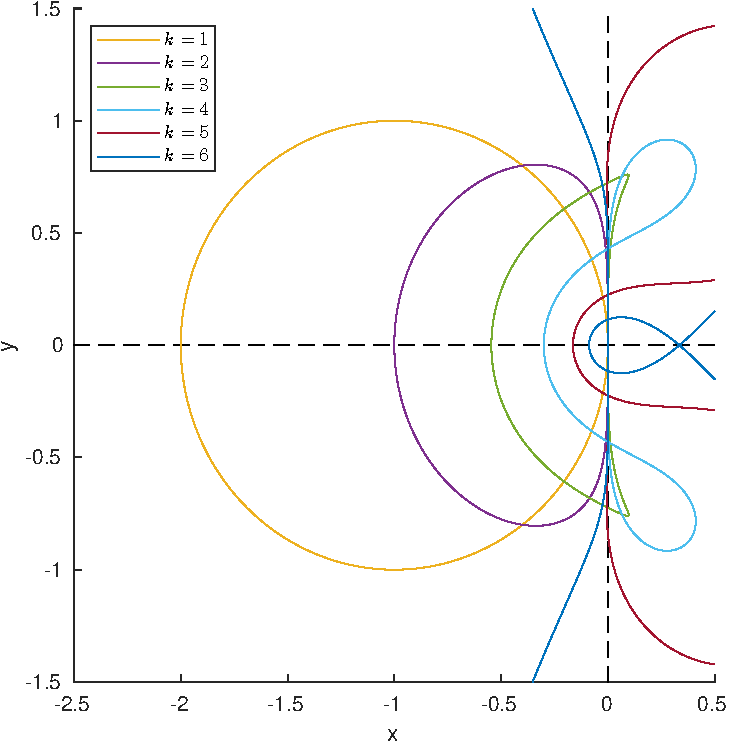
\includegraphics[height=0.4\textheight]{adams-bashforth-boundary-loci.pdf}
\caption{Boundary loci di alcuni metodi di Adams-Bashforth.}
\label{fig:lmf-adams-bashforth-boundary-loci}
\end{figure}

\begin{figure}[p]
\centering
\begin{tikzpicture}[trim axis left]
\begin{loglogaxis}[
	xlabel={$h$},
	ylabel={$\max \norm{y(t_n)-y_n}$},
	width=0.9\textwidth,
	height=0.5\textheight,
	legend style={anchor=south east,at={(0.975,0.025)}},
	ymin=1e-19
]
\addplot table {convergenza-adams-moulton-1.dat};
\addplot table {convergenza-adams-moulton-2.dat};
\addplot table {convergenza-adams-moulton-3.dat};
\addplot table {convergenza-adams-moulton-4.dat};
\addplot table {convergenza-adams-moulton-5.dat};
\addplot table {convergenza-adams-moulton-6.dat};
\addplot[dashed, domain=1e-3:1e-1] expression {x^2};
\addplot[dashed, domain=1e-3:1e-1] expression {x^3};
\addplot[dashed, domain=1e-3:1e-1] expression {0.5*x^4};
\addplot[dashed, domain=1e-3:1e-1] expression {0.25*x^5};
\addplot[dashed, domain=1e-3:1e-1] expression {max(2.2e-16,0.2*x^6)};
\addplot[dashed, domain=1e-3:1e-1] expression {max(2.2e-16,0.15*x^7)};
\legend{$k=1,O(h^2)$\\$k=2,O(h^3)$\\$k=3,O(h^4)$\\
        $k=4,O(h^5)$\\$k=5,O(h^6)$\\$k=6,O(h^7)$\\}
\end{loglogaxis}
\end{tikzpicture}
\caption{Verifica dell'ordine di convergenza di alcuni metodi di Adams-Moulton.}
\label{fig:lmf-adams-moulton-convergenza}
\end{figure}

\begin{figure}[p]
\centering
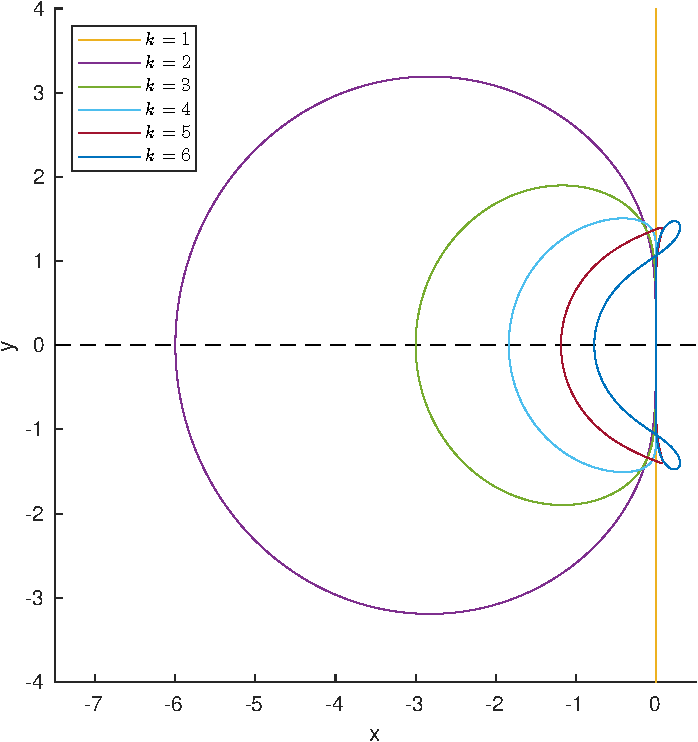
\includegraphics[height=0.4\textheight]{adams-moulton-boundary-loci.pdf}
\caption{Boundary loci di alcuni metodi di Adams-Moulton.}
\label{fig:lmf-adams-moulton-boundary-loci}
\end{figure}

\section{Formule di Newton-Cotes}

Le \emph{formule di Newton-Cotes} sono particolari metodi lineari multistep
che si ottengono tramite approssimazione del teorema fondamentale del
calcolo integrale per mezzo di una formula di quadratura di tipo interpolatorio
con ascisse equispaziate (da cui il nome \emph{Newton-Cotes}):
\[
y(t_{n+k}) - y(t_n)
= \int_{t_n}^{t_{n+k}} f(t,y(t)) \dt
\approx h \sum_{i=0}^k \beta_i f(t_{n+i},y(t_{n+i}))
\quad \Rightarrow \quad
y_{n+k} = y_n + h \sum_{i=0}^k \beta_i f_{n+i}.
\]
Il polinomio caratteristico $\rho(z)$ di questi metodi è $z^k-1$, quindi
le formule di Newton-Cotes danno sempre luogo a metodi 0-stabili,
perché le radici di $\rho(z)$ sono tutte e sole le radici $k$-esime
dell'unità e pertanto $\rho(z)$ è un polinomio di Von Neumann.
Se $k=1$ e i coefficienti $\beta_i$ corrispondono ai pesi della formula
di quadratura dei trapezi, allora otteniamo nuovamente il metodo dei trapezi
Se $k=2$ e i coefficienti $\beta_i$ corrispondono ai pesi della formula
di quadratura di Cavalieri-Simpson, allora otteniamo il \emph{metodo di Simpson}
\[
y_{n+2} = y_n + \frac{h}{3} (f_{n+2} + 4 f_{n+1} + f_n),
\]
mentre se i coefficienti $\beta_i$ corrispondono ai pesi della formula
di quadratura dei rettangoli, allora otteniamo il \emph{metodo del mid-point}
\[
y_{n+2} = y_n + 2 h f_{n+1}.
\]
Si può dimostrare che il metodo di Cavalieri-Simpson è un metodo implicito
di ordine 4 (è infatti il metodo lineare a due passi di ordine massimo;
possiamo riconoscere i suoi polinomi caratteristici nella Tabella
\ref{tab:lmf-max-order-implicit-coefficients}) e che il metodo del mid-point
è un metodo esplicito di ordine 2. Tuttavia, si può anche dimostrare che
le regioni di assoluta stabilità di questi due metodi sono vuote,
il che suggerisce che le formule di Newton-Cotes, pur essendo convergenti
in quanto consistenti e 0-stabili, hanno in pratica pessime proprietà
di stabilità. Per questa ragione, abbiamo preferito non approfondire
l'analisi di questi metodi nell'elaborato.

\section{Backward Differentiation Formulae}

I metodi lineari a $k$ passi con $\sigma(z) = z^k$ sono detti
\emph{backward differentiation formulae} (BDF, in breve).
Questi metodi, per cui adotteremo la normalizzazione $\beta_k = 1$
anziché $\alpha_k = 1$, sono quindi impliciti per costruzione.
I coefficienti $\alpha_0,\dots,\alpha_k$ vengono scelti in modo che
il metodo abbia ordine $k$ (e non $k+1$, perché la consistenza
richiede che la somma dei coefficienti $\alpha_i$ si annulli,
e questo rappresenta un vincolo aggiuntivo). Naturalmente, non c'è garanzia
che il polinomio $\rho(z)$ così ottenuto sia di Von Neumann, e infatti
si può dimostrare che tutte le backward differentiation formulae con $k > 6$
non sono 0-stabili (e quindi nemmeno convergenti), mentre quelle con
$k \leq 6$ lo sono.
Per $k=1$ si ottiene il metodo $y_{n+1} = y_n + h f(t_{n+1},y_{n+1})$,
noto come \emph{metodo di Eulero implicito}. I polinomi caratteristici
$\rho$ dei metodi di ordine superiore sono riportati nella Tabella
\ref{tab:lmf-BDF-coefficients} fino a $k=10$, insieme all'esito
della funzione \code{is\_von\_neumann} (Programma \ref{prog:is-von-neumann},
ancora una volta eseguito in aritmetica esatta).
Tali polinomi caratteristici sono stati calcolati per mezzo del
Programma \ref{prog:BDF-coefficients}.

Come nel caso dei metodi di Adams, abbiamo verificato la correttezza
dei coefficienti $\alpha_i$ andando a risolvere il problema di Cauchy
\eqref{eq:problema-moto-circolare-uniforme} e riportando nella Figura
\ref{fig:lmf-BDF-convergenza} il grafico dell'errore della soluzione
discreta in funzione di $h$. Ancora una volta, possiamo affermare che i
dati sperimentali sono in accordo con il Teorema \ref{teor:ordine-convergenza-lmf}.
L'unica differenza che abbiamo riscontrato è che stavolta l'errore associato
ai metodi di ordine più alto ($k = 5,6$) si è fermato ben prima di $10^{-15}$,
e ha cominciato a crescere per valori di $h$ minori di $10^{-2}$.
Riteniamo che questo fenomeno sia dovuto a una maggiore instabilità numerica,
che si manifesta sotto questa forma come preludio alla totale perdita di
convergenza per $k = 7$.

Per quanto riguarda l'assoluta stabilità, la Figura \ref{fig:lmf-BDF-boundary-loci}
mostra l'aspetto dei boundary loci di tutte le BDF 0-stabili.
Stavolta, la regione di assoluta stabilità corrisponde alla componente
connessa esterna a ogni curva.
In accordo con la seconda barriera di Dahlquist, solo i metodi con $k \leq 2$
sono assolutamente stabili: gli altri 4, pur avendo una regione di assolta
stabilità illimitata, non sono A-stabili per alcuni valori di $q \in \C^-$.
Osserviamo che la regione di assoluta stabilità diventa sempre più
piccola al crescere di $k$, e che per $k=6$ assume una forma piuttosto bizzarra,
con un lungo collo a sinistra dell'origine.
Questo è un esempio di regione di assoluta stabilità non convessa,
che causa il fenomeno poco intuitivo per cui la riduzione del passo $h$
può portare all'uscita di $q$ da $\mathcal{D}$ e alla conseguente
perdita del corretto comportamento asintotico del metodo numerico.
L'uso di BDF di ordine elevato non è quindi indicato nel caso di
dinamiche dissipative particolarmente oscillanti attorno al punto
di equilibrio.

\lstinputlisting[float=p, label=prog:BDF-coefficients,
caption={Calcolo dei coefficienti $\alpha_i$ e $\beta_i$ delle
backward differentiation formulae a $k$ passi.}]{BDF_coefficients.m}

\begin{table}[p]
\caption{Polinomi caratteristici $\rho$ delle backward
differentiation formulae a $k$ passi.}
\label{tab:lmf-BDF-coefficients}
\vspace*{-2.5ex}
\begin{equation*}
\begin{array}{clc}
\toprule
k & \rho(z) & \text{\code{is\_von\_neumann}} \\
\midrule
1 & z-1 & \text{\code{true}} \\
2 & (3/2)z^2-2z+(1/2) & \text{\code{true}} \\
3 & (11/6)z^3-3z^2+(3/2)z-(1/3) & \text{\code{true}} \\
4 & (25/12)z^4-4z^3+3z^2-(4/3)z+(1/4) & \text{\code{true}} \\
5 & (137/60)z^5-5z^4+5z^3-(10/3)z^2+(5/4)z-(1/5) & \text{\code{true}} \\
6 & (49/20)z^6-6z^5+(15/2)z^4-(20/3)z^3+(15/4)z^2-(6/5)z+(1/6) & \text{\code{true}} \\
7 & (363/140)z^7 + \dots & \text{\code{false}} \\
8 & (761/280)z^8 + \dots & \text{\code{false}} \\
9 & (7129/2520)z^9 + \dots & \text{\code{false}} \\
10 & (7381/2520)z^{10} + \dots & \text{\code{false}} \\
\bottomrule
\end{array}
\end{equation*}
\end{table}

\begin{figure}[p]
\centering
\begin{tikzpicture}[trim axis left]
\begin{loglogaxis}[
	xlabel={$h$},
	ylabel={$\max \norm{y(t_n)-y_n}$},
	width=0.9\textwidth,
	height=0.5\textheight,
	legend style={anchor=south east,at={(0.975,0.025)}}
]
\addplot table {convergenza-BDF-1.dat};
\addplot table {convergenza-BDF-2.dat};
\addplot table {convergenza-BDF-3.dat};
\addplot table {convergenza-BDF-4.dat};
\addplot table {convergenza-BDF-5.dat};
\addplot table {convergenza-BDF-6.dat};
\addplot[dashed, domain=1e-3:1e-1] expression {x};
\addplot[dashed, domain=1e-3:1e-1] expression {x^2};
\addplot[dashed, domain=1e-3:1e-1] expression {0.9*x^3};
\addplot[dashed, domain=1e-3:1e-1] expression {0.7*x^4};
\addplot[dashed, domain=1e-3:1e-1] expression {0.5*x^5};
\addplot[dashed, domain=1e-3:1e-1] expression {max(2.2e-16,0.4*x^6)};
\legend{$k=1,O(h^1)$\\$k=2,O(h^2)$\\$k=3,O(h^3)$\\
        $k=4,O(h^4)$\\$k=5,O(h^5)$\\$k=6,O(h^6)$\\}
\end{loglogaxis}
\end{tikzpicture}
\caption{Verifica dell'ordine di convergenza delle backward
differentiation formulae 0-stabili.}
\label{fig:lmf-BDF-convergenza}
\end{figure}

\begin{figure}[p]
\centering
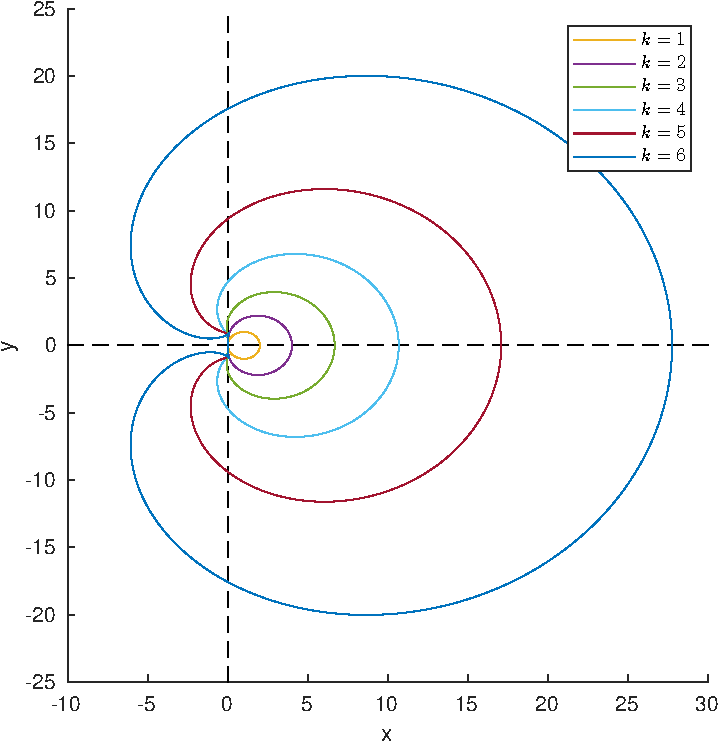
\includegraphics[height=0.4\textheight]{BDF-boundary-loci.pdf}\\
\caption{Boundary loci delle backward differentiation formulae 0-stabili.}
\label{fig:lmf-BDF-boundary-loci}
\end{figure}









